\chapter{تخمین در ابعاد بالا با رویکرد هندسی}
\label{ch:HDE}
\newpage
\section{مقدمه}
در این بخش یک چارچوب هندسی جهت حل مساله‌ی تخمین در ابعاد بالا بیان گردیده است. همچنین با ارایه‌ی تصویر شهودی از هندسه ابعاد بالا، نتایج هندسه‌ی محدب مجانبی
\LTRfootnote{asymptotic convex geometry}
 مساله‌ی تخمین و نتایج هندسی مقایسه شده است. نظریه‌های مطرح شده با کاربرد در بازیابی تنک، تکمیل ماتریس، کوانتیزه کردن، رگرسیون خطی و منطقی و مدل خطی عمومی، توضیح داده شده است. 
\subsection{تخمین مقید}
در این بخش،  چهارچوب ریاضی مساله‌ی تخمین با استفاده از قیود در ابعاد بالا بیان گردیده است. در این مساله، هدف تخمین نقطه‌ی 
$\bm{x}$
با استفاده از تعداد کمی نمونه‌ی مستقل به صورت 
$y_1,\cdots,y_m$
است که در یک مجموعه‌ی شدنی مشخص
$\mathcal{K} \subseteq \R^{n}$
قرار می‌گیرد. نقطه‌ی 
$\bm{x}$
می‌تواند نشان‌دهنده‌ی یک سیگنال در پردازش سیگنال، یک پارامتر از توزیع در آمار و یا یک ماتریس نامشخص در تکمیل ماتریس باشد. مجموعه‌ی شدنی
$\mathcal{K} $
دارای خصوصیاتی است که انتظار می‌رود سیگنال
$\bm{x}$
داشته باشد و یا ما بر آن سیگنال تحمیل می‌کنیم.


هندسه‌ی ابعاد بالای مجموعه‌ی شدنی
\LTRfootnote{feasible set}
$\mathcal{K} $
، کلید درک مساله‌ی تخمین است. یک شهود قدرتمند در رابطه با شکل مجموعه‌ها در ابعاد بالا در حوزه‌ای که با نام هندسه‌ی محدب مجانبی شناخته می‌شود، ارائه شده است
\cite{ball1997elementary,brazitikos2014geometry}.
شهود ارائه شده منجربه  نتایج بسیار دقیقی شده که برخی از آن‌ها قابل استفاده در مساله‌ی تخمین هستند. هدف اصلی از این بخش در سه موضوع زیر خلاصه می‌گردد.
\begin{itemize}
\item{
ارائه‌ی یک شهود از هندسه‌ی ابعاد بالا‌ی مجموعه
}
\item{
بیان نتایج هندسه‌ی محدب مجانبی و تایید شهود ارائه شده
}
\item{
ایجاد پیوند بین مساله‌ی تخمین در ابعاد بالا و هندسه‌ی ابعاد بالا
}
\end{itemize}

قبل از ارائه نتایج اصلی در این قسمت چند مثال کاربردی از تخمین بیان شده است.  یک کلاس ویژه از مسایل تخمین مقید در حوزه‌ی حسگری فشرده طبقه‌بندی می‌گردند. در این دسته از مسایل 
$\mathcal{K}$
دارای خاصیت تنکی  و  در برخی موارد تنکی ساختار یافته است که در آن تنها برخی مقادیر مجاز به غیر صفر شدن هستند
\cite{rao2011tight}.


یک مثال دیگر از مساله‌ی تخمین مقید، مساله‌ی تکمیل ماتریس است
\cite{recht2010guaranteed,candes2010power}.
در این مساله، 
$\mathcal{K}$
شامل ماتریس‌های رتبه پایین است و نمونه‌ها درایه‌های ماتریس هستند.

در حالت کلی، لزومی مبنی بر خطی بودن مشاهدات نیست. به عنوان یک مثال خوب می‌توان به حسگری فشرده‌ی تک بیتی اشاره نمود که در آن از یک مدل غیر خطی استفاده شده است. به صورت عمومی می‌توان مدل 
$\mathbb{E} y_{i} = \theta (\langle\bm{a}_{i}, \bm{x}\rangle)$
را برای نمونه برداری در نظر گرفت
\cite{ai2014one,plan2013robust}.

در علم آمار، این کلاس از مساله‌ی تخمین را می‌توان به صورت رگرسیون خطی (برای مشاهدات همراه با نویز)، رگرسیون منطقی (برای مشاهدات باینری) و مدل عمومی (برای مشاهدات غیر خطی)،  تفسیر نمود.

تمامی مثال‌های بیان شده در ادامه به صورت دقیق بررسی شده است. با این حال، هدف اصلی از این بخش، ارائه‌ی یک مدل فراگیر جهت استفاده در یک مجموعه‌‌ی شدنی عمومی است.

\section{مساله‌ی تخمین در ابعاد بالا}
فرض کنید که می‌خواهیم سیگنال مجهول 
$\bm{x}$
را تخمین بزنیم. فرض می‌کنیم که نمونه‌برداری به صورت تصادفی و مستقل  با استفاده از یک توزیع وابسته به 
$\bm{x}$
به صورت زیر اخذ شده است.
\begin{align}
\label{eq:eq12}
y_{i} \sim \text{distribution} (\bm{x}), \quad i= 1,\cdots,m 
\end{align}

بنابراین ما در پی بازیابی سیگنال 
$\bm{x}\in \R^{n}$
از بردار مشاهدات 
$\bm{y}\in \R^{m}$
هستیم. 
\subsection{ساختار‌های با پیچیدگی پایین}
در بسیاری از مواقع ما یک سری ویژگی برای بردار 
$\bm{x}$
در نظر می‌گیریم و یا حتی در برخی از مواقع بر آن تحمیل می‌کنیم.  می‌توان اطلاعات اضافه را به صورت زیر فرمول‌بندی نمود.
\begin{align*}
\bm{x} \in \mathcal{K}
\end{align*}
که در آن 
$\mathcal{K}$
یک مجموعه‌ی ثابت و زیرمجموعه‌ی 
$\R^{n}$
است که آن را مجموعه‌ی شدنی می‌نامیم. این  یک فرض بسیار عمومی و انعطاف‌پذیر است. در این مرحله هیچ خاصیت ویژه‌ای برای 
$\mathcal{K}$
در نظر نمی‌گیریم. به عنوان مثال می‌توان مجموعه‌ی 
$\mathcal{K}$
را تنک فرض نمود. 

شکل 
\ref{fig4}
\cite{Plan2016}
مساله‌ی تخمین را توصیف می‌کند. نمونه‌برداری می‌تواند به صورت یک نگاشت از 
$\bm{x} \in \mathcal{K}$
به 
$\bm{y} \in \R^{n}$
فرض شود و تخمین یک نگاشت از 
$\bm{y} \in \R^{n}$
به 
$\hat{\bm{x}} \in \mathcal{K}$
است که در حالت ایده‌آل معکوس نگاشت نمونه‌برداری است.

\begin{figure}
\centering
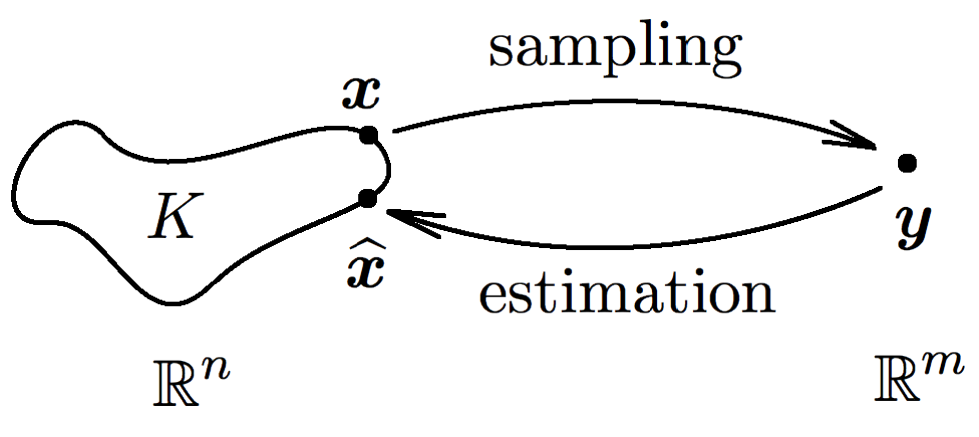
\includegraphics[scale=0.25]{Images/ch2/fig4.png}
\caption{توصیف گرافیکی مساله‌ی نمونه‌برداری و تخمین \cite{Plan2016}}
\label{fig4}
\end{figure}

اولین سوالی که به ذهن خطور می‌کند این است که اطلاعات و فرضیات موجود در مجموعه‌ی
$\mathcal{K}$
در ابعاد بالا چه کمکی به حل مساله می‌کند؟ جهت روشن شدن پاسخ مثال زیر را در نظر بگیرید. بردار 
$\bm{x}$،
$n$
بعد و بردار 
$\bm{y}$،
$m$
بعد دارد. قاعدتا، تخمین بردار 
$\bm{x}$
از
$\bm{y}$
با استفاده از 
\begin{align*}
m = O\left( n \right)
\end{align*}
مشاهده امکان‌پذیر است. حال فرض کنید که محدودیت 
$\bm{x} \in \mathcal{K}$
اضافه گردد. اگر 
$\mathcal{K}$
دارای بعد جبری
$\text{dim}(\mathcal{K})=d$
پایین باشد
$d \ll n$
، در این صورت 
$\bm{x}$
،
$d$
درجه‌ی آزادی خواهد داشت. بنابراین در این حالت تخمین با استفاده از نمونه‌های کمتر نیز امکان‌پذیر خواهد بود.
\begin{align*}
m = O\left( d \right)=o\left( n \right)
\end{align*}

این موضوع که مجموعه‌ی شدنی دارای بعد جبری کوچک باشد، به ندرت اتفاق می‌افتد. برای مثال، مجموعه‌ی تمام بردار‌های 
$s$-تنک
در 
$\R^{n}$
دارای بعد 
$n$
است. با این وجود، شهود در رابطه با بعد-پایین معتبر است. مجموعه‌های شدنی طبیعی، همانند تصاویر و ماتریس مجاورت شبکه، به نظر می‌رسد که دارای بعد پایین باشند. مجموعه‌ی
$\mathcal{K}$
ممکن است که دارای بعد بالا باشد ولی در حقیقت 
\textbf{بعد موثر}\LTRfootnote{Effective dimenstion}
آن پایین است. در ادامه‌ی این بخش،‌ با استفاده از این شهود موارد زیر بررسی شده است.
\begin{itemize}
\item{
تعیین کمیت پیچیدگی برای زیرمجموعه‌های 
$\mathcal{K}$
در 
$\R^{n}$
}
\item{
ثابت کردن امکان تخمین با استفاده از نمونه‌های کمتر از بعد جبری 
$\mathcal{K}$
}
\item{
طراحی تخمین‌گر جهت بازیابی سیگنال
}
\end{itemize}

در بخش بعدی شکل مجموعه‌ی 
$\mathcal{K}$
در ابعاد بالا ، با استفاده از ابزار‌های هندسه‌ی محدب مجانبی بررسی شده است.

\section{مقدمه‌ای بر هندسه‌ی محدب ابعاد بالا}
هندسه‌ی محدب ابعاد بالا، شکل اجسام
\LTRfootnote{Bodies}
 محدب را برای مقادیر زیاد 
$n$
بررسی می‌کند. اجسام محدب، مجموعه‌های محدب بسته، کراندار و توپر هستند. این حوزه از ریاضی، برخی اوقات هندسه‌ی محدب مجانبی و آنالیز تابعی هندسی
\LTRfootnote{Geometric functional analysis}
نیز نامیده می‌شود
\cite{ball1997elementary,brazitikos2014geometry,pisier1999volume}.


سوال اصلی در هندسه‌ی محدب ابعاد بالا این است که 
\textit{جسم محدب به چه شکل است؟}
به عنوان یک پاسخ اولیه می‌توان گفت که جسم محدب
$\mathcal{K}$
دارای یک تنه
\LTRfootnote{Bulk}
و تعدادی شاخک 
\LTRfootnote{Outlier}
است. بخش عمده‌ی حجم 
$\mathcal{K}$
در داخل تنه قرار دارد ولی معمولا قطر آن کم است. از طرف دیگر شاخک‌ها حجم کمی دارند ولی در هنگام محاسبه‌ی قطر، مقدار زیادی را به خود اختصاص می‌دهند.

با مقیاس نمودن 
$\mathcal{K}$
، تنه معمولا به شکل یک توپ اقلیدسی و شاخک‌ها به صورت نازک و بلند از توده به سمت خارج کشیده شده است. شکل
\ref{fig5}
نمایش هایپربولیک برای اجسام ابعاد بالا را نشان می‌دهد.
\begin{figure}
\centering
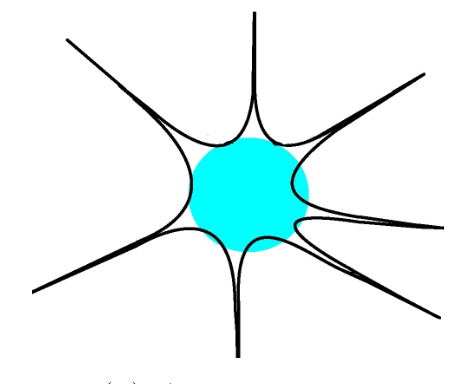
\includegraphics[scale=0.3]{Images/ch2/fig5.png}
\caption{نمایش هایپربولیک مجموعه‌های محدب ابعاد بالا\cite{Plan2016}}
\label{fig5}
\end{figure}

نمایش نشان داده شده در شکل
\ref{fig5}
محدب به نظر نمی‌رسد ولی به خوبی خواص ذکر شده را به تصویر می‌کشد. به عنوان مثال توپ نُرم 
$\ell_1$
را در نظر بگیرید. در این حالت مجموعه‌ی 
$\mathcal{K}$
به صورت زیر تعریف می‌گردد.
\begin{align*}
\mathcal{K}= B^{n}_{1}=\lbrace\bm{x} \in \R^{n}: \norm{\bm{x}}_{1}\leq 1 \rbrace
\end{align*}
در این حالت توپ اقلیدسی محاط در 
$\mathcal{K}$
را با 
$B$
نشان می‌دهیم. این توپ دارای قطر 
$2/\sqrt{n}$
است. می‌توان نشان داد که حجم
$B$
و 
$\mathcal{K}$
به صورت زیر قابل مقایسه هستند.
\begin{align*}
\text{vol}_{n} \left( B \right)^{1/n}\asymp \text{vol}_{n} \left( \mathcal{K} \right)^{1/n} \asymp \dfrac{1}{n}
\end{align*}
بنابراین، 
$B$
تشکیل دهنده‌ی تنه‌ی
$\mathcal{K}$
است و به صورت تقریبی بیشتر حجم 
$\mathcal{K}$
را تشکیل می‌دهد(شکل
\ref{fig6}). 

\begin{figure}
\centering
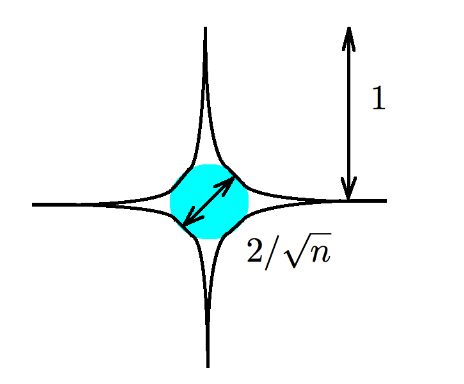
\includegraphics[scale=0.35]{Images/ch2/fig6.png}
\caption{نمایش ابعاد بالا‌ی توپ 
$l_{1}$
\cite{Plan2016}}
\label{fig6}
\end{figure}


\subsection{تمرکز حجم}
در این قسمت تحلیل ریاضی تایید‌کننده‌ی شهود مطرح شده در قسمت قبلی تحت عنوان تمرکز حجم 
\LTRfootnote{Concentration of volume}
بیان شده است.  فرض کنید که مجموعه‌ی
$\mathcal{K}$
ایزوتروپیک باشد. یعنی برای یک بردار تصادفی انتخاب شده از 
$\mathcal{K}$
با توزیع یکنواخت، میانگین برابر صفر و ماتریس کوواریانس همانی باشد. به عبارت ریاضی
\begin{align*}
\mathbb{E}~ \bm{x} = 0 , \quad \mathbb{E} ~\bm{x}\bm{x}^{T} = \bm{I}_{n}.
\end{align*}
با محاسبه‌ی رد ماتریس در دو طرف معادله‌ی دوم در رابطه‌ی فوق داریم:
\begin{align*}
\mathbb{E}~ \norm{\bm{x}}_2^2 = n
\end{align*}
در این حالت حداقل
$90$
 درصد از حجم 
$\mathcal{K}$
 در یک توپ اقلیدسی با اندازه‌ی 
 $O(\sqrt{n})$
 قرار دارد.
 تمرکز حجم در ابعاد بالا به صورت قضیه‌ی زیر خلاصه می‌گردد.
\begin{theorem}
\label{theorem:thm2}
\cite[قضیه~3.2]{vershynin2015estimation}
فرض کنید
$\mathcal{K}$
یک جسم ایزوتروپیک در
$\R^{n}$
 و 
$\bm{x}$
یک بردار تصادفی باشد که با توزیع یکنواخت از 
$\mathcal{K}$
انتخاب شده است. برای بردار 
$\bm{x}$
داریم:
\begin{itemize}
\item{
(تمرکز حجم)
به ازای یک $t>1$ 
\begin{align}
\mathbb{P}\lbrace\norm{\bm{x}}_{2}>t\sqrt{n} \rbrace \leq \exp\left( -ct\sqrt{n}\right)
\end{align}
}
\item{
(پوسته‌ی نازک)
برای هر 
$\epsilon \in (0,1)$
یکی 
\begin{align}
\mathbb{P}\lbrace\vert \norm{\bm{x}}_{2}-\sqrt{n}\vert > \epsilon\sqrt{n} \rbrace \leq C \exp\left( -c\epsilon^{3}\sqrt{n}\right)
\end{align}
}
\end{itemize}
\end{theorem}
\begin{proof}
 قضیه‌ی فوق در 
\cite{paouris2006concentration}
اثبات شده است.
\end{proof}

تعبیر هندسی تنه و شاخک به ما کمک می‌کند که بتوانیم یک برش تصادفی از 
$\mathcal{K}$
را تصور کنیم. فرض کنید که 
$E$
یک زیرفضای تصادفی از
$\R^{n}$
با بعد ثابت
$d$
باشد. در این حالت اگر
$d$
به اندازه‌ی کافی کوچک باشد، انتظار داریم که 
$E$
از تنه‌ی
$\mathcal{K}$
عبور کند و با شاخک‌ها برخورد نداشته باشد. به این ترتیب 
$\mathcal{K}\cap E$
خود یک توپ خواهد بود (شکل
\ref{fig7}).
قضیه‌ی دیورتزکی
\LTRfootnote{Dvoretzky}
این موضوع را به صورت ریاضی بیان می‌کند.
\begin{figure}
\centering
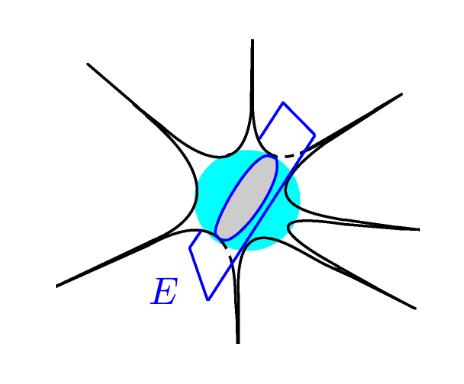
\includegraphics[scale=0.35]{Images/ch2/fig7.png}
\caption{نمایش ابعاد بالا‌ی  
$\mathcal{K}\cap E$
\cite{Plan2016}}
\label{fig7}
\end{figure}

\begin{theorem}
\label{theorem:thm3}
\cite[قضیه~3.3]{vershynin2015estimation}
فرض کنید 
$\mathcal{K}$
یک مجموعه‌ی محدب متقارن نسبت به مبدا، در 
$\R^n$
باشد. در این صورت بیضی محاط در 
$\mathcal{K}$
که بیشترین حجم را دارد توپ واحد اقلیدسی است. با فرض مقدار ثابت
$\epsilon \in (0,1)$
و انتخاب 
$d = c \epsilon^{-2} \log n$
بعد به صورت تصادفی از توزیع گرسمنین
\LTRfootnote{Grassmanian}
به عنوان زیرفضای
$E$
،یک 
$R\geq 0$
وجود دارد که با احتمال بالا (بیش از ۹۹ درصد)، رابطه‌ی زیر برقرار است.
\begin{align}
\left(1-\epsilon \right)RB^2_n \subseteq \mathcal{K}\cap E \subseteq \left(1+\epsilon \right)RB^2_n 
\end{align}
\end{theorem}
\begin{proof}
اثبات این قضیه در 
\cite{brazitikos2014geometry}
آورده شده است.
\end{proof}

بر خلاف تعبیر مشخص تقاطع یک جسم محدب با یک زیرفضای تصادفی با ابعاد پایین،‌ در حالتی که زیر فضای مورد نظر دارای بعد بالا باشد، نمی‌توان به سادگی شهود مشخصی برای تقاطع ارائه نمود. با این وجود می‌توان قطر این تقاطع را محاسبه نمود. یک کران برای این قطر تحت عنوان کران
$M^{\ast}$ 
ارائه شده است. قبل از بیان قضیه چند تعریف مقدماتی نیاز است که در ادامه بیان شده است.

\subsection{عرض میانگین}
با استفاده از عرض میانگین
\LTRfootnote{Mean width}
می‌توان مشخصات هندسی مهم یک مجموعه در 
$\R^n$
را به دست آورد. 
یک زیرمجموعه‌ی محدود 
$\mathcal{K}$
از 
$\R^n$
را فرض کنید ( محدب بودن، بسته و توپر بودن لازم نیست). عرض 
$\mathcal{K}$
در جهت مشخص
$\hat{\bm{n}}\in S^{n-1}$
به صورت کمترین فاصله‌ی بین دو ابرصفحه با بردار نرمال
$\bm{n}$
که شامل 
$\mathcal{K}$
است، تعریف می‌گردد. به عنوان مثال در شکل
\ref{fig8}
فاصله در جهت
$\hat{\bm{n}}$
برابر با 
$d$
است. به صورت تحلیلی، عرض در جهت 
$\bm{x}$
به صورت زیر تعریف می‌گردد.
\begin{align}
	\sup_{\bm{u},\bm{v}\in \mathcal{K}} \langle \hat{\bm{n}}, \bm{u}-\bm{v}  \rangle
\end{align}

\begin{figure}
\centering
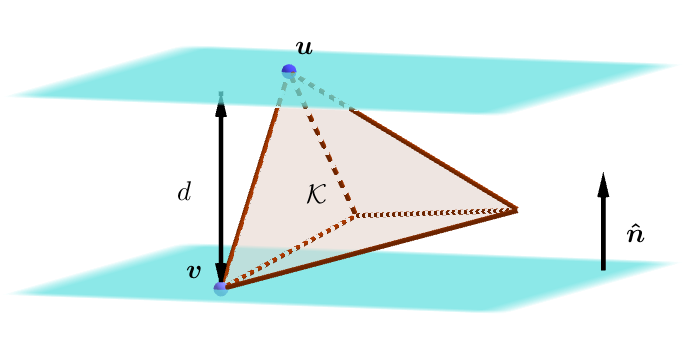
\includegraphics[scale=0.35]{Images/ch2/fig8.png}
\caption{عرض   
$\mathcal{K}$
در جهت
$\hat{\bm{n}}$
}
\label{fig8}
\end{figure}


اگر 
$\hat{\bm{n}}$
به صورت تصادفی با توزیع یکنواخت از 
$S^{n-1}$
انتخاب گردد، آنگاه عرض میانگین کروی
\LTRfootnote{spherical mean width}
مجموعه‌ی
$\mathcal{K}$
به صورت زیر تعریف می‌گردد.
\begin{align} 
\label{eq:eq13}
\tilde{w}\left(\mathcal{K}\right) := \mathbb{E} \sup_{\bm{u},\bm{v}\in \mathcal{K}} \langle \hat{\bm{n}}, \bm{u}-\bm{v}  \rangle
\end{align} 

در حوزه‌های دیگر همچون احتمال ابعاد بالا و تئوری یادگیری آماری، بسیار مرسوم است که بردار تصادفی با توزیع کروی
$\hat{\bm{n}} \sim \text{Unif}(S^{n-1})$
با یک بردار تصادفی نرمال استاندارد 
$\bm{g} \sim N (0,I_n)$
جایگزین گردد. برتری بردار
$\bm{g}$
نسبت به بردار
$\hat{\bm{n}}$
، درایه‌های مستقل آن است. عرض میانگین گوسی به صورت زیر تعریف می‌گردد.
\begin{definition}[عرض میانگین گوسی]
فرض کنید که 
$\bm{g} \sim N (0,I_n)$
بردار تصادفی نرمال استاندارد در
$\R^{n}$
باشد. در این صورت عرض میانگین گوسی یک مجموعه‌ی کراندار
$\mathcal{K}$
در 
$\R^{n}$
به صورت زیر تعریف می‌گردد.
\begin{align}
\label{eq:eq14}
w\left(\mathcal{K}\right) := \mathbb{E} \sup_{\bm{u},\bm{v}\in \mathcal{K}} \langle \bm{g}, \bm{u}-\bm{v}  \rangle
\end{align}	
\end{definition}
جهت خلاصه‌نویسی از این به بعد بجای عرض میانگین گوسی، از عبارت عرض گوسی استفاده می‌کنیم.


در نگاه اول مشخص است که عرض گوسی با ضریب 
$\sqrt{n}$
از عرض کروی بزرگتر است. با فرض
$\hat{\bm{n}}$
به صورت
$\hat{\bm{n}}= \bm{g} / \norm{\bm{g}}_{2}$
، می‌توان عرض  کروی را به صورت زیر بازنویسی نمود. 
\begin{align}
\tilde{w}\left(\mathcal{K}\right) := \mathbb{E} \sup_{\bm{u},\bm{v}\in \mathcal{K}} \langle \bm{g} / \norm{\bm{g}}_{2}, \bm{u}-\bm{v}  \rangle
\end{align}
با توجه به اینکه اندازه و جهت  بردار تصادفی نرمال از یکدیگر مستقل هستند، رابطه‌ی بین عرض کروی و عرض میانگین را می‌توان به صورت زیر نوشت.
\begin{align}
w\left(\mathcal{K}\right) =  \mathbb{E} \norm{\bm{g}}_{2} \tilde{w}\left(\mathcal{K}\right).
\end{align} 
در ادامه مقدار عرض میانگین برای چند مجموعه‌ی پرکاربرد آورده شده است.
\begin{latin}
\begin{itemize}
\item{$\mathcal{K}:= B_{2}^{n}$ or $S^{n-1} \Longrightarrow w\left(\mathcal{K}\right) =\mathbb{E} \norm{\bm{g}}_{2} \leq \sqrt{n}$ }
\item{$\mathcal{K} \subseteq B_{2}^{n}$ linear algebraic dimension $d \Longrightarrow w\left(\mathcal{K}\right)\leq 2\sqrt{d} $.}
\item{$\mathcal{K}$ consist of all unit $s$-sparse vectors in $\R^{n}\Longrightarrow c\sqrt{s \log(2n/s)} \leq w\left(\mathcal{K}\right) \leq C\sqrt{s \log(2n/s)} $} 
\end{itemize}
\end{latin}

با توجه به اینکه مجموعه‌های مورد استفاده‌ی ما در بسیاری از حالات مجموعه‌های محدب هستند، جهت محاسبه‌ی عرض میانگین می‌توان از برنامه‌های بهینه‌سازی محدب استفاده نمود.
همان‌گونه که در ابتدای این بخش بیان گردید، هدف از ارائه‌ی عرض میانگین، به دست آوردن خواص تقاطع یک مجموعه و یک زیر فضای تصادفی با بعد بالا معرفی گردید. قضیه
\ref{theorem:thm4}
مقدار قطر 
$\mathcal{K}\cap E$
را با استفاده از عرض میانگین محدود می‌کند.
\begin{theorem}
\label{theorem:thm4}
\cite[قضیه~3.12]{vershynin2015estimation}
فرض کنید 
$\mathcal{K}$
یک مجموعه‌ی محدود در
$\R^{n}$
و 
$E$
یک زیرفضای تصادفی با توزیع گرسمنین از
$\R^{n}$
با متمم بعد 
$m$
باشد. در این صورت قطر 
$\mathcal{K}\cap E$
به صورت زیر محدود می‌گردد.
\begin{align}
\label{eq:eq15}
\mathbb{E}~ \text{diam}\left( \mathcal{K}\cap E \right) \leq \dfrac{C w\left(\mathcal{K}\right)}{\sqrt{m} }
\end{align}

\end{theorem} 

\section{بررسی تخمین‌گر با رویکرد هندسی}
پس از بیان مقدمات هندسه‌ی ابعاد بالا، در این بخش دوباره به مساله‌ی تخمین در ابعاد بالا باز می‌گردیم. هدف اصلی این بخش، ارائه‌ی یک شهود از مساله‌ی تخمین ابعاد بالا با استفاده از مطالب بیان شده است.

همانگونه که در بخش ابتدایی این فصل بیان گردید، در مساله‌ی تخمین هدف پیدا نمودن بردار مجهول
$\bm{x} \in \mathcal{K} \subseteq \R^{n}$
با استفاده از مشاهدات خطی به صورت 
\begin{align}
\label{eq:eq16}
\bm{y} = \bm{A}\bm{x}
\end{align} 
است. در معادله‌ی فوق ماتریس
$\bm{A}\in \R^{m\times n}$
، یک ماتریس تصادفی با درایه‌های گرفته شده از توزیع نرمال استاندارد است. همانگونه که بیان گردید در حسگری فشرده، تعداد نمونه‌ها از بعد بردار 
$\bm{x}$
کمتر است یا به عبارت دیگر 
$m<n$.
دقت کنید که از بردار 
$\bm{x}$
اطلاعات زیر موجود است.
\begin{itemize}
\item{
$\bm{x}$
در یک زیرفضای تصادفی افاین
\LTRfootnote{Affine}
صدق می‌کند.(
$\bm{x}^{\prime}~:~ \bm{A}\bm{x}^{\prime}=\bm{y}$
)
}
\item{
$\bm{x}$
در یک مجموعه‌ی مشخص
$\mathcal{K}$
صدق می‌کند.
}
\end{itemize}

بنابراین با استفاده از این اطلاعات، یک تخمین مناسب از 
$\bm{x}$
، انتخاب
$\hat{\bm{x}}$
از تقاطع مجموعه‌ی دارای دو شرط فوق است. شکل
\ref{fig9}
تقاطع میان این دو مجموعه را نشان می‌دهد. همانگونه که از شکل مشخص است، در این حالت با توجه به شرط تخمین‌گر می‌توان پاسخ را انتخاب نمود. خطای تخمین در این حالت برابر با بیشترین فاصله‌ی بین دو نقطه از محل تقاطع است. این فاصله برابر با قطر تقاطع مجموعه‌ی
$\mathcal{K}$
و زیرفضای افاین
$\bm{x}^{\prime}~:~ \bm{A}\bm{x}^{\prime}=\bm{y}$
است. با استفاده از قضیه‌ی
\eqref{theorem:thm4}
می‌توان یک کران برای حداکثر خطا به دست آورد. در قضیه‌ی
\eqref{theorem:thm5}
مقدار کران خطا برای تخمین‌گر حساب شده است.


\begin{figure}
\centering
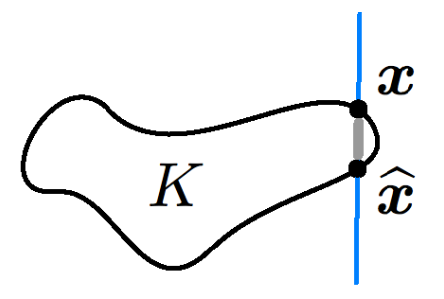
\includegraphics[scale=0.35]{Images/ch2/fig9.png}
\caption{
$\hat{\bm{x}}$
پاسخ تخمینی بردار
$\bm{x}$
از محل تقاطع 
$\mathcal{K}$
و 
زیرفضای افاین
$\bm{x}^{\prime}~:~ \bm{A}\bm{x}^{\prime}=\bm{y}$
\cite{Plan2016}}
\label{fig9}
\end{figure}


\begin{theorem}
\label{theorem:thm5}
\cite[قضیه~ ۴.۱]{vershynin2015estimation}
فرض کنید
$\mathcal{K}\subset \R^{n}$
یک مجموعه‌ی کراندار، 
$\bm{x}\in \mathcal{K}$
بردار مجهول و
$\bm{y}= \bm{A}\bm{x}$
بردار مشاهدات باشند.
با انتخاب بردار
$\hat{\bm{x}}$
با استفاده از هر تخمین‌گر که در دو رابطه‌ی
$\hat{\bm{x}}\in \mathcal{K}$
و
$\bm{y}= \bm{A}\hat{\bm{x}}$
صدق کند. رابطه‌ی زیر برقرار خواهد بود.
\begin{align}
\label{eq:eq17}
\mathbb{E}~ \sup_{\bm{x}\in \mathcal{K}} \norm{\hat{\bm{x}}-\bm{x}}_{2} \leq \dfrac{C w\left(\mathcal{K}\right)}{\sqrt{m}}
\end{align}
\end{theorem}
\begin{proof}
اثبات این قضیه در 
\cite{vershynin2015estimation}
آمده است.
\end{proof}


\subsection{تخمین با استفاده از مساله‌ی بهینه‌سازی}
در این قسمت با ساده‌تر کردن دو فرض
$\hat{\bm{x}}\in \mathcal{K}$
و
$\bm{y}= \bm{A}\hat{\bm{x}}$
، تخمین‌گر را به صورت یک مساله‌ی بهینه‌سازی در نظر می‌گیریم. علاوه بر این فرض کنید که مجموعه‌ی
$\mathcal{K}$
توپر و ستاره شکل باشد. ستاره شکل بودن به این معنا است که به ازای هر نقطه‌ی موجود در 
$\mathcal{K}$
، یک پاره خط وجود دارد که تماما در داخل مجموعه قرار دارد و از مرکز به آن نقطه متصل می‌گردد. به عبارت ریاضی:
\begin{align*}
t\mathcal{K} \subseteq \mathcal{K} \quad \text{for all} \quad t \in [0,1].
\end{align*}

برای چنین مجموعه‌ی شدنی، می‌توان با تغییر مقدار 
$t$
از صفر به سمت یک، مجموعه‌ی
$t\mathcal{K}$
را از یک نقطه تا حدی بزرگ نمود که به زیر فضای
$\bm{x}^{\prime}~:~ \bm{A}\bm{x}^{\prime}=\bm{y}$
مماس گردد. در این حالت می‌توان نقطه‌ی تماس بین مجموعه‌ی
$t\mathcal{K}$
و زیرفضا را به عنوان پاسخ تخمین‌گر در نظر گرفت. در شکل 
\ref{fig10}
این فرآیند  به صورت گرافیکی نمایش داده است.

\begin{figure}
\centering
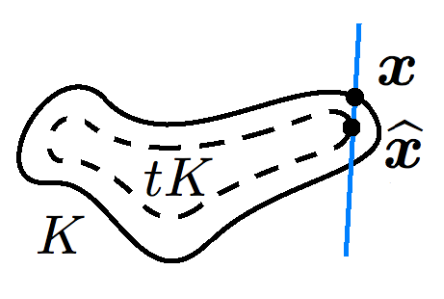
\includegraphics[scale=0.35]{Images/ch2/fig10.png}
\caption{
$\hat{\bm{x}}$
پاسخ تخمینی بردار
$\bm{x}$
از محل تقاطع 
$t\mathcal{K}$
و 
زیرفضای افاین
$\bm{x}^{\prime}~:~ \bm{A}\bm{x}^{\prime}=\bm{y}$
\cite{Plan2016}}
\label{fig10}
\end{figure}


جهت توضیح ریاضی، نیاز به تعریف تابع مینکوسکی
\LTRfootnote{Minkowski}
است. تابع مینکوسکی
به هر نقطه‌ی
$\bm{x}\in \R^{n}$
یک مقدار غیر منفی 
$\norm{\bm{x}}_{\mathcal{K}}$
اختصاص می‌دهد که به صورت زیر تعریف می‌گردد.
\begin{align}
\label{eq:eq18}
\norm{\bm{x}}_{\mathcal{K}} = \inf \lbrace \lambda >0~:~ \lambda^{-1}\bm{x}\in \mathcal{K}\rbrace
\end{align}

تابع مینکوسکی در آنالیز تابعی هندسی و آنالیز محدب پر کاربرد است. ویژگی‌های تابع مینکوسکی در مرجع 
\cite{rockafellar1970convex}
بیان شده است. در این قسمت ما تنها به صورت خلاصه به بیان خواص مورد نیاز خود می‌پردازیم. اول اینکه تابع
$\bm{x}\mapsto \norm{\bm{x}}_{\mathcal{K}}$
دارای خاصیت همگنی است (
$\norm{a\bm{x}}_{\mathcal{K}} = a \norm{\bm{x}}_{\mathcal{K}}; a>0$).
خاصیت دیگر تابع مینکوسکی
به صورت زیر بیان می‌شود.
\begin{align}
\label{eq:eq19}
\mathcal{K}= \lbrace \bm{x}~:~ \norm{\bm{x}}_{\mathcal{K}}\leq 1 \rbrace
\end{align}
در صورتی که مجموعه‌ی
$\mathcal{K}$
محدب باشد، تابع مینکوسکی
برابر با تابع نُرم خواهد بود. در قضیه‌ی
\eqref{theorem:thm6}
یک کران برای خطای حاصل از استفاده از این تخمین‌گر بیان شده است.
\begin{theorem}
\label{theorem:thm6}
\cite[قضیه~ ۴.۲]{vershynin2015estimation}
فرض کنید
$\hat{\bm{x}}$
پاسخ بهینه‌سازی زیر باشد.
\begin{align}
\label{eq:eq20}
\min \norm{\bm{x}^{\prime}}_{\mathcal{K}} \quad \text{s.t.} \quad \bm{A}\bm{x}^{\prime}= \bm{y}
\end{align}
آنگاه داریم
\begin{align}
\label{eq:eq21}
\mathbb{E}~ \sup_{\bm{x}\in \mathcal{K}} \norm{\hat{\bm{x}}-\bm{x}}_{2} \leq \dfrac{C w\left(\mathcal{K}\right)}{\sqrt{m}}
\end{align}
\end{theorem}
\begin{proof}
اثبات این قضیه در 
\cite{vershynin2015estimation}
آورده شده است.
\end{proof}

\subsection{بعد موثر}
فرض کنید در رابطه‌ی
\eqref{eq:eq21}
مقدار خطا به صورت زیر محدود گردد.
\begin{align}
\label{eq:eq22}
\mathbb{E}~ \sup_{\bm{x}\in \mathcal{K}} \norm{\hat{\bm{x}}-\bm{x}}_{2} \leq 0.01
\end{align}
در این صورت تعداد
\begin{align}
\label{eq:eq23}
m \sim O\left( w\left(\mathcal{K} \right)^{2}\right)
\end{align}
نمونه کافی خواهد بود. مقدار مربع عرض میانگین
$w\left(\mathcal{K} \right)^{2}$،
نشان دهنده‌ی عرض موثر مجموعه‌ی شدنی 
$\mathcal{K}$
است. بنابراین همانگونه که در بخش‌های مقدماتی از این فصل بیان گردید، با استفاده از ویژگی بعد موثر، می‌توان تعداد نمونه‌ی لازم جهت بازیابی صحیح را به دست آورد.

\section{نمونه‌برداری تک-بیتی از دیدگاه هندسی}
همانگونه که در فصل
\ref{ch:intro}
بیان گردید، با فرض نمونه‌برداری به صورت
\eqref{eq:eq10}،
اطلاعات دامنه از بین می‌رود. در این صورت می‌توان سیگنال مورد نظر را به صورت نرمالیزه در نظر گرفت. یعنی:
\begin{align}
\norm{\bm{x}}_{2}=1
\end{align}
در این حالت مجموعه‌ی شدنی 
$\mathcal{K}$
برابر با کره‌ی اقلیدسی واحد
$S^{n-1}$
می‌گردد. با فرض 
$\bm{a}_{i}$
به عنوان سطر 
$i$ام 
از ماتریس
$\bm{A}$
، می‌توان آن را به عنوان بردار نرمال یک ابرصفحه نیز در نظر گرفت. هر مولفه از بردار اندازه‌گیری (
$y_{i}$)
در این حالت، برابر با علامت ضرب داخلی بردار نرمال صفحه خواهد بود.
\begin{align}
y_{i} = \text{sign}(\langle\bm{a}_{i}, \bm{x}\rangle)
\end{align}
واضح است که اگر زاویه‌ی بین بردار
$\bm{x}$
و بردار نرمال صفحه از ۹۰ درجه کمتر باشد، علامت ضرب داخلی مثبت است و در غیر این صورت منفی خواهد بود. بنابراین هر نمونه، مشخص کننده‌ی یک نیم فضا خواهد بود. با اضافه شدن شرط 
$\norm{\bm{x}}_{2}=1$
فضای پاسخ به صورت بخشی از پوسته‌ی 
$S^{n-1}$
خواهد بود. در شکل
\ref{fig11}
تعبیر هندسی این مساله در فضای
$\R^{3}$
و به ازای
$m=4$
نشان داده شده است. اگر دو بردار دلخواه
$\bm{u}\in \R^{3}$
و
$\bm{v}\in \R^{3}$
بر روی 
$S^{2}$
فرض گردد، با استفاده از قضیه‌ی برش ابرصفحه‌های تصادفی می‌توان حداکثر فاصله‌ی بین دو نقطه را بر حسب تعداد نمونه‌های اخذ شده محدود نمود.

\begin{figure}
\centering
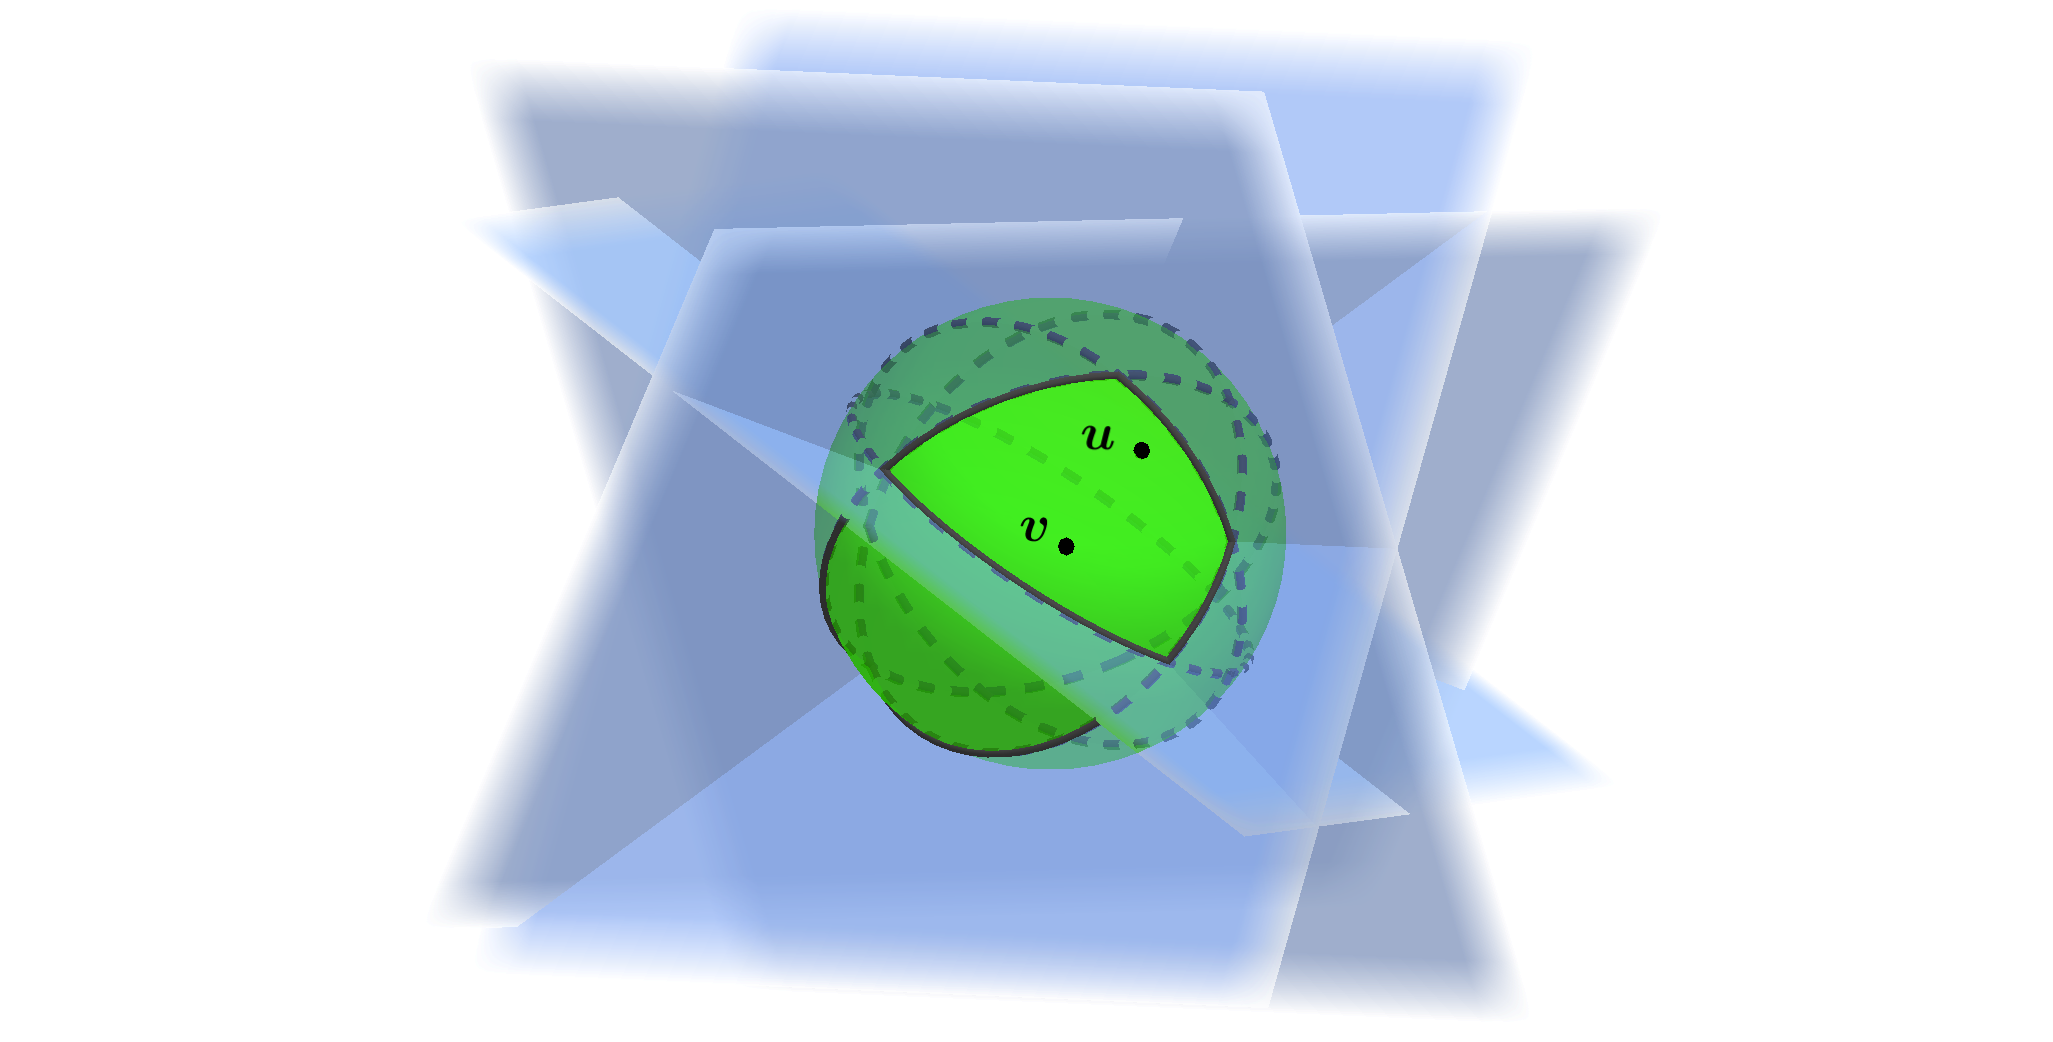
\includegraphics[scale=1.3]{Images/ch2/fig11.png}
\caption{تعبیر هندسی نمونه‌برداری تک بیتی
در 
$\R^3$
. با استفاده از قضیه‌ی برش ابرصفحه تصادفی می‌توان فاصله‌ی بین دو بردار تصادفی 
$\bm{v}$
و
$\bm{u}$
را محدود نمود.}
\label{fig11}
\end{figure}

\subsection{برش ابرصفحه تصادفی}
همانگونه که بیان گردید، هر یک از نمونه‌های باینری نشان دهنده‌ی یک نیم فضا است که با اضافه شدن شرط نرمالیزه بودن بردار، تشکیل یک مجموعه‌ی شدنی می‌دهند. سوالی که مطرح می‌گردد این است که چه تعداد نمونه‌ی جهت بازیابی سیگنال با خطای مشخص لازم است؟

در مرجع
\cite{plan2014dimension}
اندازه‌ی برش‌های تشکیل شده بر روی یک مجموعه‌ی شدنی بر حسب تعداد نمونه بررسی شده است. این مرجع، فرآیند تقسیم پوسته‌ی 
$S^{n-1}$
به برش‌های مختلف را برش ابر صفحه تصادفی
\LTRfootnote{Random Hyperplane Tessellation}
(به اختصار
\lr{RHT}
)
نامیده است.


قبل از بیان نتیجه اصلی مرجع
\cite{plan2014dimension}
، لازم است که تعریف برش 
$ \delta $-یکنواخت
را بیان نمود.

\begin{definition}
\cite[تعریف~1.1]{plan2014dimension}
\label{defn:D-UT}
فرض کنید که 
$\mathcal{K}$
یک زیر مجموعه از
$ S^{n-1} $
باشد. همچنین
$m$
ابرصفحه در
$\R^{n}$
فرض کنید. 
$ d\left(\bm{u},\bm{v}\right) $
نشان دهنده‌ی نسبت تعداد ابرصفحه‌هایی است که دو نقطه‌ی 
$ \bm{u}$
و
$\bm{y}$
در
$\mathcal{K} $
را از یکدیگر جدا می‌کند. 
مجموعه‌ی 
$\mathcal{K}$
را برش
$ \delta $-یکنواخت
می‌گوییم اگر برای یک مقدار 
$\delta >0$
رابطه‌ی زیر برقرار باشد.
\begin{align}
\label{eq:eq24}
|d\left(\bm{v},\bm{u}\right)-d_{G}\left(\bm{v},\bm{u}\right) |\leq \delta \quad \bm{u},\bm{v} \in \mathcal{K}
\end{align}
\end{definition}

با توجه به مساله‌ی مورد بررسی، با فرض سطر‌های 
$\bm{A}$
به عنوان بردار نرمال صفحات، 
$d\left(\bm{v},\bm{u}\right)$
نشان‌دهنده‌ی فاصله‌ی همینگ نرمالیزه‌ی (
$ d_{H}\left(\bm{z},\bm{t}\right)  $
)
بین
$\bm{z}:= \text{sign}\left(\bm{A}\bm{u}\right)$
و
$\bm{t}:= \text{sign}\left(\bm{A}\bm{v}\right)$
است.  در قضیه‌ی
\eqref{theorem:thm7}
تعداد نمونه‌های لازم جهت برش
$ \delta $-یکنواخت
، را بر حسب بعد موثر مجموعه‌ی
$\mathcal{K}$
محاسبه شده است.
\begin{theorem}
\label{theorem:thm7}
\cite[قضیه~1.2]{plan2014dimension}
فرض کنید
$\mathcal{K}\subset S^{n-1}$
، 
$\delta>0$
و
\begin{align*}
	m \geq C \delta^{-6} w\left(\mathcal{K}\right)^{2}
\end{align*}
باشد.
در این صورت با در نظر گرفتن یک دسته‌ی 
$m$تایی
از ابرصفحه‌های تصادفی تولید شده با توزیع یکنواخت، با احتمال 
$1-2\exp(-c\delta^{2}m)$
، این صفحات یک برش
$ \delta $-یکنواخت
از  مجموعه‌ی 
$\mathcal{K}$
ایجاد می‌کنند. 
\end{theorem}
در بخش بعدی از این پایان‌نامه با استفاده از قضیه‌ی فوق باند خطای بازیابی سیگنال‌های دیکشنری-تنک با نمونه‌های باینری، محاسبه شده است. 












